% AntRoute - dokumentacja projektu
% Plik jest napisany w prostym LaTeX, aby pandoc dobrze zamienił go na Word:
%   pandoc antroute_dokumentacja.tex -o antroute_dokumentacja.docx --toc
% (uruchom w katalogu docs/latex, aby ścieżki do rysunków były poprawne)

\documentclass[11pt,a4paper]{article}

\usepackage[utf8]{inputenc}
\usepackage[T1]{fontenc}
\usepackage[polish]{babel}
\usepackage{lmodern}
\usepackage[margin=2.5cm]{geometry}
\usepackage{amsmath}
\usepackage{amssymb}
\usepackage{graphicx}
\usepackage{booktabs}
\usepackage{longtable}
\usepackage{hyperref}

\title{AntRoute: planowanie trasy zwiedzania omijającej tłok\\
algorytmem mrówkowym z antyferomonem}
\author{Marcin Wolder}
\date{Opis projektu, stan na 5 listopada 2026 r.}

\begin{document}

\maketitle

\begin{abstract}
AntRoute planuje jednodniową pieszą trasę po Manhattanie, która odwiedza wartościowe miejsca w godzinach, gdy jest w nich mało ludzi. Problem to Time-Dependent Orienteering Problem (TDOP) z karą za tłok. Profile tłoku powstają z prawdziwych danych Foursquare (227\,428 check-inów z Nowego Jorku). Solver to Ant Colony System (ACS) z antyferomonem, przeszukiwaniem lokalnym i ponownym planowaniem po zdarzeniu ogłoszonym w trakcie dnia (skok tłoku, zamknięcie miejsca, wypadek lub parada). Pierwsza wersja programu (PoC) jest gotowa i przetestowana: 46 testów automatycznych, ok. 39\,000 uruchomień w 14 eksperymentach. Główna metoda (ACS z przeszukiwaniem lokalnym) ma średnią lukę 0,19\% do najlepszego znanego rozwiązania, a dla 25 miejsc 0,09\% do rozwiązania dokładnego z solvera CP-SAT. Metoda zachłanna ma lukę 18\%. Dokument opisuje problem, dane, model, algorytm, implementację, wyniki, ograniczenia i plan dalszych prac.
\end{abstract}

\tableofcontents

% =====================================================================
\section{Wprowadzenie}

\subsection{Problem}

Osoba, która zwiedza miasto, chce w ciągu jednego dnia odwiedzić wartościowe miejsca: muzea, kawiarnie, parki, restauracje. Chce też uniknąć tłoku. Tłok w miejscu zmienia się w ciągu dnia. Może też nagle wzrosnąć przez zdarzenie, na przykład darmowe wejście do muzeum. Miejsce może być nieoczekiwanie zamknięte, a ulica zablokowana przez wypadek albo paradę.

Przykład: popularne muzeum warto odwiedzić o 10:00, a nie o 15:00, gdy ma szczyt. Gdy o 10:23 zdarzy się wypadek na drodze, którą trasa ma przejść o 11:30, plan na resztę dnia trzeba zmienić.

\subsection{Cel projektu}

AntRoute układa trasę, która:
\begin{itemize}
  \item odwiedza miejsca poza ich godzinami szczytu,
  \item uwzględnia preferencje użytkownika (np. więcej kultury, mniej zakupów),
  \item reaguje na zdarzenia znane rano i na zdarzenia ogłoszone w trakcie dnia,
  \item mieści się w budżecie czasu i wraca do punktu startu.
\end{itemize}

Cele szczegółowe:
\begin{enumerate}
  \item Zbudować godzinowe profile tłoku miejsc z prawdziwych danych check-in.
  \item Zaimplementować ACS dla TDOP z karą za tłok i antyferomonem.
  \item Dodać symulowane zdarzenia: skok tłoku, zamknięcie miejsca, utrudnienie w ruchu.
  \item Pokazać, jak zdarzenie zmienia trasę i feromon: przed zdarzeniem, w trakcie i po nim.
  \item Porównać ACS z prostymi metodami (algorytm zachłanny, trasa losowa) i z rozwiązaniem dokładnym.
\end{enumerate}

\subsection{Wejście i wyjście}

\begin{table}[h]
\centering
\caption{Dane wejściowe planera.}
\begin{tabular}{ll}
\toprule
Wejście & Przykład \\
\midrule
Punkt startu & Times Square (40,7580; $-73{,}9855$) \\
Godzina startu $T_0$ & 08:00 \\
Budżet czasu $T_{max}$ & 8 h \\
Preferencje $u_c$ & persona ,,Turysta kulturalny'' albo własne wagi kategorii \\
Typ dnia & dzień roboczy lub weekend \\
Scenariusz zdarzeń & plik YAML \\
\bottomrule
\end{tabular}
\end{table}

Wynik to uporządkowana lista miejsc z godziną przybycia, czasem pobytu, tłokiem i zyskiem, a dla scenariusza ze zdarzeniem także trasa bez zdarzenia do porównania.

\subsection{Poza zakresem}

\begin{itemize}
  \item Prawdziwe dane o tłoku w czasie rzeczywistym (zdarzenia są symulowane).
  \item Aplikacja mobilna i nawigacja krok po kroku.
  \item Transport publiczny (model zakłada ruch pieszo).
\end{itemize}

% =====================================================================
\section{Podstawy teoretyczne}

\subsection{Orienteering Problem i jego wersja zależna od czasu}

Orienteering Problem (OP) to problem wyboru i kolejności wierzchołków grafu: każdy wierzchołek daje zysk, przejście między wierzchołkami kosztuje czas, a łączny czas trasy nie może przekroczyć budżetu. Celem jest maksymalny łączny zysk. OP jest NP-trudny, więc dokładne metody działają tylko dla małych instancji.

W wersji zależnej od czasu (TDOP) zysk wierzchołka albo czas przejścia zależą od godziny. W AntRoute zysk miejsca zależy od tłoku w chwili przybycia, a czas przejścia zależy od utrudnień w ruchu. Wartość miejsca zależy więc od całej wcześniejszej części trasy.

\subsection{Ant Colony System}

Ant Colony System (ACS) to algorytm mrówkowy Dorigo i Gambardelli [2]. Kolonia sztucznych mrówek buduje rozwiązania krok po kroku. Wybór następnego wierzchołka zależy od feromonu $\tau$ (pamięć kolonii o dobrych wyborach) i heurystyki $\eta$ (lokalna ocena wyboru). ACS ma trzy cechy:
\begin{enumerate}
  \item regułę pseudolosową: z prawdopodobieństwem $q_0$ mrówka wybiera najlepszy lokalnie wierzchołek, w przeciwnym razie losuje proporcjonalnie do $\tau \cdot \eta^\beta$,
  \item lokalną aktualizację feromonu po każdym kroku, która zmniejsza feromon na użytej krawędzi i zwiększa różnorodność,
  \item globalną aktualizację tylko na najlepszej trasie.
\end{enumerate}
Montemanni i Gambardella [3] zastosowali ACS do Team Orienteering Problem z oknami czasowymi.

\subsection{Antyferomon}

Antyferomon to sygnał odwrotny do feromonu: odstrasza mrówki od złych wyborów. Montgomery i Randall [4] pokazali, że antyferomon może poprawić eksplorację, ale zbyt silny pogarsza wyniki. W AntRoute antyferomon $\varphi_j(b)$ jest na miejscu $j$ i zależy od 30-minutowego przedziału dnia $b$, więc to samo muzeum może mieć duży $\varphi$ o 11:00 i mały o 17:00.

\subsection{ACO dla problemów dynamicznych}

Guntsch i Middendorf [5] badali, jak zmienić feromon, gdy problem zmienia się w trakcie obliczeń. Strategia ,,restart'' wyrównuje feromon w kierunku wartości początkowej: kolonia nie zaczyna od zera, ale nie jest też przywiązana do starego rozwiązania. AntRoute używa tej strategii przy ponownym planowaniu (ciepły start).

% =====================================================================
\section{Dane}

\subsection{Źródło}

Projekt używa publicznego zbioru Foursquare NYC and Tokyo Check-in Dataset [1], plik \texttt{dataset\_TSMC2014\_NYC.txt}. Zbiór ma 227\,428 check-inów z Nowego Jorku, 1\,083 użytkowników, 38\,333 miejsc i 251 kategorii, z okresu od kwietnia 2012 do lutego 2013 r. Plik to TSV bez nagłówka (kodowanie ISO-8859-1) z 8 kolumnami: identyfikator użytkownika, identyfikator miejsca, identyfikator i nazwa kategorii, szerokość i długość geograficzna, przesunięcie strefy czasowej, czas UTC. Strona zbioru nie podaje licencji, więc projekt używa go tylko do celów akademickich, a plik nie jest w repozytorium. Wielokąt Manhattanu pochodzi z NYC Open Data [6].

\subsection{Przygotowanie danych}

\begin{enumerate}
  \item Przelicz czas UTC na czas lokalny: czas lokalny = UTC + przesunięcie strefy.
  \item Odrzuć check-iny poza Manhattanem (test punktu w wielokącie).
  \item Zostaw tylko 11 kategorii o różnych godzinach szczytu (tabela poniżej).
  \item Policz histogram 24 godzin dla każdej kategorii, osobno dla dni roboczych i weekendu.
  \item Wygładź histogram cykliczną średnią kroczącą z oknem 3 h (23:00 łączy się z 0:00).
  \item Znormalizuj profil do zakresu $[0,1]$: $P_c(h) = n_c(h) / \max_h n_c(h)$.
  \item Wybierz miejsca z co najmniej 10 check-inami (774 miejsca na Manhattanie).
  \item Policz wagę wartości miejsca: $w_i = \log(1+n_i) / \max_j \log(1+n_j)$.
  \item Policz czasy przejścia pieszo: odległość haversine $\times\,1{,}3$ (siatka ulic), prędkość 5 km/h.
\end{enumerate}

Poprawność kroku 1 sprawdza test automatyczny: histogram godzinowy dla całego Nowego Jorku musi być równy tabeli referencyjnej z dokumentacji. Różnica wynosi 0 dla wszystkich $11 \times 24$ liczb.

\begin{table}[h]
\centering
\caption{Wybrane kategorie miejsc na Manhattanie (wszystkie dni) i założone czasy pobytu.}
\begin{tabular}{lrrrr}
\toprule
Kategoria & Check-iny & Miejsca & Miejsca $\geq 10$ check-inów & Pobyt [min] \\
\midrule
Breakfast Spot & 209 & 41 & 8 & 45 \\
Coffee Shop & 4\,866 & 440 & 160 & 20 \\
Bakery & 856 & 176 & 20 & 15 \\
Museum & 95 & 28 & 2 & 90 \\
Art Museum & 260 & 27 & 5 & 120 \\
Park & 2\,862 & 222 & 44 & 45 \\
Clothing Store & 2\,280 & 649 & 51 & 30 \\
American Restaurant & 2\,178 & 387 & 55 & 75 \\
Movie Theater & 1\,353 & 63 & 26 & 150 \\
Mexican Restaurant & 1\,455 & 204 & 47 & 60 \\
Bar & 10\,574 & 1\,374 & 356 & 60 \\
\bottomrule
\end{tabular}
\end{table}

\subsection{Profile tłoku}

Profil $P_c(h)$ opisuje względny tłok kategorii $c$ w godzinie $h$. Dane są za rzadkie na profil dla każdego miejsca (mediana to 2 check-iny na miejsce), więc wszystkie miejsca jednej kategorii mają ten sam kształt profilu. Różnicę między miejscami dają waga $w_i$ i zdarzenia.

Małe kategorie mają zaszumione profile. Reguła awaryjna: gdy para (kategoria, typ dnia) ma mniej niż 100 check-inów, profil pochodzi z wszystkich dni, a gdy to za mało, ze wspólnej grupy Museum i Art Museum. Na Manhattanie Museum ma tylko 95 check-inów, więc używa profilu grupy. Breakfast Spot w weekend używa profilu z wszystkich dni.

Zbiór nie ma godzin otwarcia. Model przyjmuje, że miejsce jest zamknięte, gdy $P_c(t) < 0{,}05$.

\begin{figure}[h]
\centering
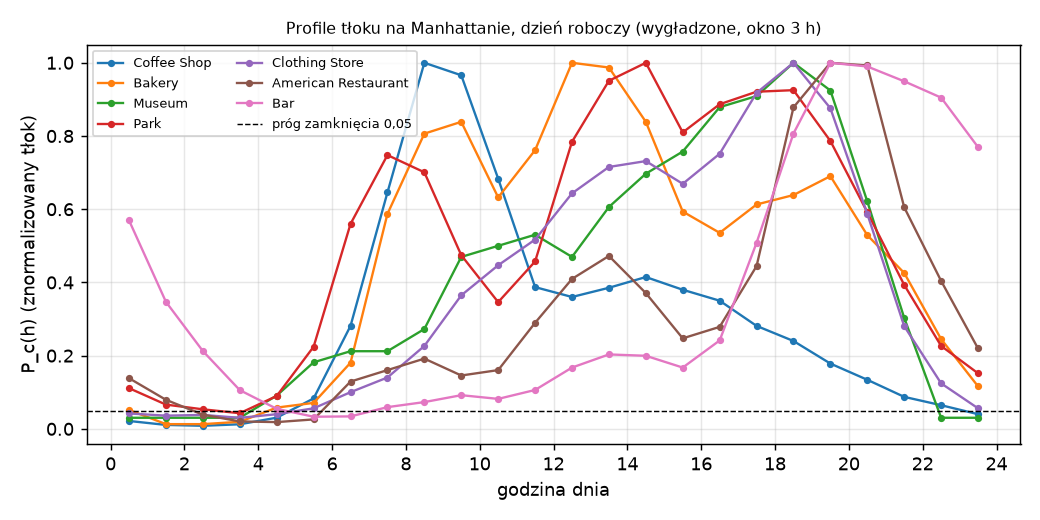
\includegraphics[width=0.9\textwidth]{figures/profiles.png}
\caption{Profile tłoku wybranych kategorii (dzień roboczy). Linia przerywana to próg zamknięcia 0,05.}
\end{figure}

\subsection{Wersje danych (bootstrap)}

Aby sprawdzić stabilność wyników, program tworzy 20 wersji profili metodą bootstrap: losuje dni ze zwracaniem i liczy profil od nowa. Każda wersja symuluje inny ,,typowy dzień''.

% =====================================================================
\section{Model matematyczny}

\subsection{Oznaczenia}

\begin{table}[h]
\centering
\caption{Oznaczenia modelu.}
\begin{tabular}{lll}
\toprule
Symbol & Znaczenie & Jednostka \\
\midrule
$V = \{0, 1, \ldots, N\}$ & wierzchołki; 0 = punkt startu i końca & - \\
$t_{ij}(t)$ & czas przejścia pieszo z $i$ do $j$ przy wyjściu w chwili $t$ & min \\
$s_i$ & czas pobytu w miejscu $i$ & min \\
$c(i)$ & kategoria miejsca $i$ & - \\
$w_i$ & wartość miejsca, $[0,1]$ & - \\
$P_c(t)$ & profil tłoku kategorii $c$, $[0,1]$ & - \\
$E_i(t)$ & dodatkowy tłok ze zdarzenia & - \\
$C_i(t)$ & łączny tłok w miejscu $i$ & - \\
$u_c$ & preferencja użytkownika dla kategorii $c$, $[0,1]$ & - \\
$\lambda$ & siła kary za tłok, $[0,1]$ & - \\
$T_0$, $T_{max}$ & godzina startu, budżet czasu & min \\
$K_c$ & maksymalna liczba miejsc kategorii $c$ w trasie & - \\
$a_i$ & czas przybycia do miejsca $i$ & min \\
\bottomrule
\end{tabular}
\end{table}

\subsection{Tłok i zysk}

Tłok ma dwie części: tło z danych i zdarzenia scenariusza:
\begin{equation}
C_i(t) = P_{c(i)}(t) + E_i(t).
\end{equation}
Zysk z miejsca maleje, gdy tłok rośnie:
\begin{equation}
S_i(a_i) = u_{c(i)} \cdot w_i \cdot \bigl(1 - \lambda \cdot \min(1, C_i(a_i))\bigr).
\end{equation}
Profil $P_c(t)$ jest liniowo interpolowany między punktami w środkach godzin (wartość $P_c(h)$ należy do chwili $h$:30), cyklicznie przez północ. Dzięki temu zysk nie skacze o pełnej godzinie.

Domyślnie $\lambda = 0{,}8$. Gdy $\lambda = 0$, model ignoruje tłok. Gdy $\lambda = 1$, miejsce w szczycie nie daje zysku. Gdy $u_c = 0$, kategoria $c$ nie trafia do trasy.

\subsection{Funkcja celu i ograniczenia}

Trasa to ciąg $r = (0, v_1, \ldots, v_k, 0)$. Czas przybycia:
\begin{equation}
a_{v_1} = T_0 + t_{0 v_1}(T_0), \qquad a_{v_{j+1}} = a_{v_j} + s_{v_j} + t_{v_j v_{j+1}}\bigl(a_{v_j} + s_{v_j}\bigr).
\end{equation}
Cel:
\begin{equation}
\max_r \sum_{j=1}^{k} S_{v_j}(a_{v_j}).
\end{equation}
Ograniczenia:
\begin{enumerate}
  \item Budżet czasu: powrót do punktu 0 najpóźniej o $T_0 + T_{max}$.
  \item Każde miejsce jest w trasie najwyżej raz.
  \item Miejsce jest otwarte przez cały pobyt: $P_c(t) \geq 0{,}05$ dla $t \in [a_i, a_i + s_i]$ i brak zdarzenia ,,zamknięcie'' w tym czasie.
  \item Różnorodność: najwyżej $K_c$ miejsc kategorii $c$ (domyślnie 1, dla restauracji 2).
\end{enumerate}
Model nie pozwala na czekanie przed miejscem.

Ograniczenie 3 jest sprawdzane dokładnie. $P_c$ jest odcinkami liniowe, więc jego minimum na przedziale pobytu leży na końcu przedziału albo w węźle interpolacji wewnątrz przedziału. Program sprawdza tylko te punkty.

\subsection{Dlaczego algorytm mrówkowy}

\begin{itemize}
  \item OP jest NP-trudny, więc dokładne metody działają tylko dla małych $N$.
  \item Zysk zależy od godziny przybycia. ACS buduje trasę krok po kroku i w każdym kroku zna aktualną godzinę, więc heurystyka może liczyć zysk dla prawdziwego czasu przybycia.
  \item Feromon i antyferomon to pamięć kolonii. Gdy zdarzenie zmienia problem w trakcie dnia, kolonia nie zaczyna od zera, tylko dostosowuje tę pamięć.
  \item Algorytm nie wymaga treningu. Feromon ,,uczy się'' tylko w trakcie jednego uruchomienia.
\end{itemize}

% =====================================================================
\section{Algorytm}

\subsection{Budowa trasy przez jedną mrówkę}

\begin{enumerate}
  \item Ustaw mrówkę w punkcie startu. Ustaw zegar $t = T_0$.
  \item Wyznacz zbiór dozwolonych miejsc $F(i)$. Miejsce $j$ jest dozwolone, gdy: nie było odwiedzone, jest otwarte przez cały pobyt, limit $K_c$ nie jest przekroczony i mrówka zdąży wrócić do punktu 0 w budżecie.
  \item Jeżeli $F(i)$ jest pusty, wróć do punktu 0 i zakończ trasę.
  \item Wybierz następne miejsce $j$ regułą wyboru.
  \item Zastosuj lokalną aktualizację feromonu na krawędzi $(i, j)$. Jeżeli tłok w $j$ przekracza próg $\theta$, dodaj antyferomon.
  \item Ustaw $t \leftarrow t + t_{ij}(t) + s_j$. Przejdź do kroku 2.
\end{enumerate}

\subsection{Reguła wyboru}

Heurystyka to zysk na minutę dla prawdziwej godziny przybycia:
\begin{equation}
\eta_{ij}(t) = \frac{S_j\bigl(t + t_{ij}(t)\bigr)}{t_{ij}(t) + s_j}.
\end{equation}
Niech $b_j$ oznacza 30-minutowy przedział dnia, w którym mrówka przybędzie do $j$. Z prawdopodobieństwem $q_0$ mrówka wybiera miejsce z największą wartością $\tau_{ij}\,\eta_{ij}(t)^\beta\,(1 + \varphi_j(b_j))^{-\gamma}$. W przeciwnym razie losuje miejsce z rozkładu:
\begin{equation}
p_{ij} = \frac{\tau_{ij}\,\eta_{ij}(t)^{\beta}\,\bigl(1 + \varphi_j(b_j)\bigr)^{-\gamma}}{\sum_{l \in F(i)} \tau_{il}\,\eta_{il}(t)^{\beta}\,\bigl(1 + \varphi_l(b_l)\bigr)^{-\gamma}}.
\end{equation}

\subsection{Aktualizacja feromonu}

Lokalna aktualizacja po każdym kroku mrówki:
\begin{equation}
\tau_{ij} \leftarrow (1 - \psi)\,\tau_{ij} + \psi\,\tau_0.
\end{equation}
Globalna aktualizacja po każdej iteracji, tylko na krawędziach najlepszej trasy od początku obliczeń (także na krawędzi powrotu):
\begin{equation}
\tau_{ij} \leftarrow (1 - \rho)\,\tau_{ij} + \rho \cdot Profit_{best}.
\end{equation}
Wartość początkowa: $\tau_0 = Profit_{greedy} / N$, gdzie $Profit_{greedy}$ to zysk trasy zachłannej. Pierwsza wersja dokumentacji proponowała $\tau_0 = (N \cdot Profit_{greedy})^{-1}$, przez analogię do $(n \cdot L_{nn})^{-1}$ w ACS dla TSP. W TSP depozyt to odwrotność długości, a w OP depozyt to zysk, więc ta analogia daje złą skalę: stosunek depozytu do $\tau_0$ wynosi ok. $N \cdot Profit^2$, a nie $N$ jak w TSP. Wzór $Profit_{greedy}/N$ zachowuje stosunek $N$. Program zawiera obie wersje (parametr \texttt{tau0\_mode}), a eksperyment E4 je porównuje.

\subsection{Antyferomon}

Feromon $\tau_{ij}$ jest na krawędziach i przyciąga mrówki. Antyferomon $\varphi_j(b)$ jest na miejscach i odstrasza mrówki. Indeks $b$ to 30-minutowy przedział (96 przedziałów, czyli 48 h, bo trasa może zacząć się o 20:00 i trwać 12 h).

\begin{table}[h]
\centering
\caption{Źródła antyferomonu.}
\begin{tabular}{lll}
\toprule
Źródło & Kiedy & Wartość \\
\midrule
Skok tłoku & w przedziałach zdarzenia & $\varphi_j^E(b) = \varphi_{max} \cdot E_j(b)$ \\
Zamknięcie miejsca & przedziały w oknie zamknięcia & $\varphi_j^E(b) = \varphi_{max}$ \\
Utrudnienie w ruchu & przedziały w oknie, miejsca w obszarze & $\varphi_j^E(b) = \varphi_{max}(1 - 1/m)$ \\
Mrówki & wizyta z tłokiem $C_j(a_j) > \theta$ & $\varphi_j^A(b) \mathrel{+}= \Delta\varphi \cdot C_j(a_j)$ \\
\bottomrule
\end{tabular}
\end{table}

Razem $\varphi_j(b) = \varphi_j^E(b) + \varphi_j^A(b)$. Część od mrówek paruje po każdej iteracji: $\varphi^A \leftarrow (1 - \rho_\varphi)\,\varphi^A$. Część od zdarzenia trwa, dopóki zdarzenie trwa. Pierwsza wersja dokumentacji przewidywała antyferomon ze zdarzeń tylko dla skoku tłoku. Wiersze dla zamknięcia i utrudnienia dodano w PoC (parametr \texttt{phi\_event\_types}); ich wpływ sprawdza eksperyment E13b.

\subsection{Przeszukiwanie lokalne}

Główna metoda (ACS-LS) poprawia najlepszą trasę każdej iteracji przeszukiwaniem lokalnym z pierwszą poprawą. Ruchy:
\begin{enumerate}
  \item wstaw nieodwiedzone miejsce w dowolną pozycję,
  \item zamień miejsce w trasie na nieodwiedzone,
  \item przenieś jedno miejsce na inną pozycję,
  \item zamień dwa miejsca miejscami.
\end{enumerate}
Każdy ruch jest oceniany tą samą funkcją oceny co trasy wszystkich metod, więc trasa po przeszukiwaniu jest zawsze dozwolona. Taki krok jest standardowy w ACS dla TSP i dla TOPTW [2, 3]. Program pamięta trasy już poprawione i nie poprawia ich ponownie.

\subsection{Ponowne planowanie w trakcie dnia}

Zdarzenie ma chwilę ogłoszenia $t_a$. Gdy $t_a \leq T_0$, plan poranny od początku zna zdarzenie. Gdy $t_a > T_0$, program planuje resztę dnia od nowa:
\begin{enumerate}
  \item Weź prawdziwe czasy przybycia obecnego planu.
  \item Ustal pozycję użytkownika w chwili $t_a$. Jeżeli użytkownik jest w miejscu, kończy pobyt, a nowy start to to miejsce po pobycie. Jeżeli użytkownik jest w drodze, przejście jest przerwane (cel może być właśnie zamknięty), a nowy start to poprzednie miejsce w chwili $t_a$.
  \item Zbuduj podproblem: nowy start, reszta budżetu, odwiedzone miejsca wyłączone, limity $K_c$ pomniejszone, zdarzenia znane w chwili $t_a$.
  \item Uruchom ACS na podproblemie (domyślnie 50 iteracji).
  \item Nowy plan = wykonana część + nowa część. Oceń cały plan na prawdziwym przebiegu dnia.
\end{enumerate}

\begin{table}[h]
\centering
\caption{Warianty startu ponownego planowania.}
\begin{tabular}{lll}
\toprule
Wariant & Feromon $\tau$ na starcie & Antyferomon $\varphi$ na starcie \\
\midrule
Zimny start & $\tau_0$ na wszystkich krawędziach & tylko od zdarzeń \\
Ciepły start & $\tau \leftarrow (1-\kappa)\tau + \kappa\tau_0$ z planu porannego & od zdarzeń + od mrówek z planu porannego \\
\bottomrule
\end{tabular}
\end{table}

\subsection{Warianty i parametry}

\begin{table}[h]
\centering
\caption{Metody porównywane w eksperymentach.}
\begin{tabular}{ll}
\toprule
Metoda & Opis \\
\midrule
\texttt{random} & dodaje losowe dozwolone miejsca, aż nie ma dozwolonych \\
\texttt{greedy} & w każdym kroku wybiera miejsce z największym $\eta_{ij}(t)$ \\
\texttt{acs\_a} & ACS z antyferomonem, parametry z dokumentacji ($q_0 = 0{,}9$) \\
\texttt{acs\_b} & ACS-A z feromonem zależnym od pory dnia (8 przedziałów po 3 h) \\
\texttt{acs\_ls} & ACS-A z przeszukiwaniem lokalnym i $q_0 = 0{,}5$ (metoda główna) \\
\texttt{acs\_ls+nophi} & metoda główna bez antyferomonu ($\gamma = 0$) \\
\texttt{acs\_ls+static} & metoda główna bez kary za tłok w solverze ($\lambda = 0$) \\
\texttt{cpsat} & rozwiązanie dokładne (CP-SAT, OR-Tools) dla $N = 25$ \\
\texttt{fixed} & plan bez wiedzy o zdarzeniu, wykonany bez zmian \\
\bottomrule
\end{tabular}
\end{table}

\begin{table}[h]
\centering
\caption{Parametry algorytmu.}
\begin{tabular}{lll}
\toprule
Parametr & Wartość & Źródło \\
\midrule
liczba mrówek $m$ & 10 & [2] \\
$\beta$ & 2 & [2] \\
$q_0$ & 0,9 (\texttt{acs\_a}); 0,5 (\texttt{acs\_ls}) & [2]; strojenie E4 \\
$\rho$, $\psi$ (parowanie) & 0,1; 0,1 & [2, 3] \\
$\tau_0$ & $Profit_{greedy}/N$ & decyzja projektowa, E4 \\
$\lambda$ & 0,8 & założenie \\
$\gamma$, $\varphi_{max}$ & 1; 5 & założenie; [4] \\
$\Delta\varphi$, $\rho_\varphi$, $\theta$ & 0,5; 0,1; 0,7 & założenie \\
$\kappa$ (wyrównanie po zdarzeniu) & 0,3 & [5] \\
liczba iteracji & 2000; 50 po zdarzeniu & strojenie (zob. niżej) \\
\bottomrule
\end{tabular}
\end{table}

Pierwsza wersja dokumentacji zakładała 500 iteracji albo 60 s. Implementacja w Numba wykonuje 2000 iteracji zwykle w mniej niż 1 s, a 500 iteracji czasem kończy się przed wyjściem z optimum lokalnego. Dlatego wszystkie warianty ACS mają 2000 iteracji, co daje uczciwe porównanie przy tym samym budżecie.

\subsection{Pseudokod}

\begin{verbatim}
def acs(problem, params, seed, tau=None, phi_ants=None):
    greedy_route = greedy(problem)
    tau0 = profit(greedy_route) / N
    tau = full(tau0) if tau is None else (1 - kappa) * tau + kappa * tau0
    phi_event = event_antipheromone(problem)        # od zdarzen
    phi_ants = zeros() if phi_ants is None else phi_ants
    best = greedy_route
    for it in range(params.iterations):
        routes = [build_route(problem, tau, phi_event + phi_ants)
                  for ant in range(params.m)]       # z lokalna aktualizacja
        it_best = max(routes, key=profit)
        if params.local_search:
            it_best = local_search(problem, it_best)
        if profit(it_best) > profit(best):
            best = it_best
        global_update(tau, best, params.rho)
        phi_ants *= (1 - params.rho_phi)
    return best, tau, phi_ants
\end{verbatim}

% =====================================================================
\section{Zdarzenia i scenariusze}

Zdarzenie to symulowana zmiana warunków w mieście. Zdarzenia nie pochodzą z danych: użytkownik albo eksperyment dodaje je do scenariusza. Dane opisują tylko tłok w zwykły dzień. Każde zdarzenie ma typ, miejsce lub obszar, okno czasu $[t_s, t_e]$ i chwilę ogłoszenia $t_a$.

\begin{table}[h]
\centering
\caption{Typy zdarzeń.}
\begin{tabular}{lll}
\toprule
Typ & Przykład & Wpływ na model \\
\midrule
\texttt{crowd\_surge} & darmowe wejście do muzeum & $E_i(t) = s$ w oknie, potem $s \cdot e^{-(t - t_e)/T_d}$ \\
\texttt{closure} & remont, zamknięty lokal & miejsce niedozwolone w oknie \\
\texttt{traffic} & wypadek, parada & $t_{ij}(t) = m \cdot t_{ij}$ dla przejść przez obszar \\
\bottomrule
\end{tabular}
\end{table}

Przejście jest ,,w obszarze'', gdy odcinek między miejscami przecina koło o promieniu $r$. Mnożnik działa, gdy przejście zaczyna się w oknie zdarzenia. Duży mnożnik (np. 50) odpowiada praktycznie zamkniętej drodze.

Przykład pliku scenariusza:
\begin{verbatim}
name: all_events
day_type: weekday
events:
  - type: crowd_surge
    venue: "@top:Art Museum"     # najcenniejsze muzeum sztuki w instancji
    window: ["10:00", "13:00"]
    strength: 1.0
    decay_min: 60
    announced: "11:00"           # ogloszone w trakcie dnia
  - type: closure
    venue: "@top:Coffee Shop"
    window: ["08:00", "12:00"]
  - type: traffic
    center: [40.7536, -73.9832]
    radius_m: 400
    window: ["12:00", "15:00"]
    factor: 2.0
\end{verbatim}

% =====================================================================
\section{Program}

\subsection{Architektura}

Program to potok w Pythonie: dane $\rightarrow$ profile $\rightarrow$ instancja $\rightarrow$ solver $\rightarrow$ ocena $\rightarrow$ eksperymenty $\rightarrow$ raport. Każdy krok zapisuje wynik do pliku, więc można uruchomić każdy krok osobno. Najważniejsza zasada: zysk i ograniczenia liczy tylko jeden moduł (\texttt{evaluate.py}). Każda metoda zwraca tylko trasę, a ocena jest wspólna, więc porównanie metod jest uczciwe.

\begin{table}[h]
\centering
\caption{Moduły programu.}
\begin{tabular}{ll}
\toprule
Moduł & Zadanie \\
\midrule
\texttt{data/prepare.py} & wczytanie TSV, czas lokalny, filtr Manhattanu \\
\texttt{model/profiles.py} & profile $P_c(h)$, wygładzanie, wagi $w_i$, bootstrap \\
\texttt{model/instance.py} & wybór $N$ miejsc, macierz czasów przejścia \\
\texttt{model/evaluate.py} & jedyna funkcja oceny: $C_i$, $S_i$, $t_{ij}(t)$, ograniczenia \\
\texttt{model/problem.py} & instancja + persona + budżet + zdarzenia znane planiście \\
\texttt{scenario/events.py} & zdarzenia z plików YAML \\
\texttt{solvers/aco.py}, \texttt{kernels.py} & ACS, warianty, antyferomon, przeszukiwanie lokalne \\
\texttt{solvers/replan.py} & ponowne planowanie (zimny i ciepły start) \\
\texttt{solvers/greedy.py}, \texttt{random\_route.py} & metody porównawcze \\
\texttt{solvers/brute.py}, \texttt{exact.py} & pełny przegląd ($N \leq 8$) i CP-SAT \\
\texttt{experiments/} & konfiguracje YAML, runner równoległy \\
\texttt{report/} & wykresy i raport z wynikami \\
\bottomrule
\end{tabular}
\end{table}

\subsection{Decyzje implementacyjne}

\begin{itemize}
  \item \textbf{Wybór $N$ miejsc:} losowanie warstwowe według kategorii ze stałym ziarnem (co najmniej 1 miejsce z każdej kategorii, reszta proporcjonalnie). Ta sama instancja trafia do wszystkich metod.
  \item \textbf{Szybkość:} pętla budowy trasy, ocena trasy i przeszukiwanie lokalne są skompilowane przez Numba. ACS dla $N = 100$ i 2000 iteracji trwa zwykle poniżej 1 s.
  \item \textbf{Powtarzalność:} jedno ziarno losowania na uruchomienie; to samo ziarno daje tę samą trasę (test automatyczny).
  \item \textbf{Rozwiązanie dokładne:} CP-SAT z ograniczeniem cyklu, czasem w jednostkach 0,1 min i tabelami zysku co 1 min. Nadmiarowe ograniczenie budżetu (suma przejść i pobytów na wybranych łukach $\leq T_{max}$) wzmacnia ograniczenie górne: bez niego CP-SAT nie dowodził optimum w 60 s. Trasa z CP-SAT jest zawsze oceniana ponownie w czasie ciągłym.
  \item \textbf{Wybór celu zdarzenia w eksperymentach:} zdarzenie trafia w miejsce, które plan bez zdarzeń naprawdę odwiedza. Miejsce, którego trasa nie odwiedza, nie pokazuje reakcji.
\end{itemize}

\subsection{Testy}

Program ma 46 testów automatycznych (pytest). Pokrycie modułu oceny testami wynosi 99\%.

\begin{table}[h]
\centering
\caption{Kryteria ukończenia pierwszej wersji i ich stan.}
\begin{tabular}{lll}
\toprule
Id & Kryterium & Stan \\
\midrule
K1 & jedno polecenie uruchamia cały potok & spełnione (\texttt{run\_all.py}) \\
K2 & dane odtwarzają tabelę referencyjną check-inów & spełnione (różnica 0) \\
K3 & testy każdego wzoru i ograniczenia, pokrycie $\geq 90\%$ & spełnione (99\%) \\
K4 & ACS znajduje optimum dla $N \leq 8$ w $\geq 95\%$ uruchomień & spełnione (ACS-LS) \\
K5 & ACS lepszy od metody zachłannej (Wilcoxon) & spełnione ($p < 0{,}0001$) \\
K6 & luka do CP-SAT dla $N = 25$ $\leq 5\%$ & spełnione (0,09\%) \\
K7 & to samo ziarno daje tę samą trasę & spełnione \\
K8 & zdarzenia działają zgodnie z modelem & spełnione \\
K9 & wyniki eksperymentów z wnioskami & spełnione \\
\bottomrule
\end{tabular}
\end{table}

Testy sprawdzają między innymi: wartości wzorów policzone ręcznie, interpolację bez skoku o pełnej godzinie, wykrycie zamknięcia w środku pobytu, wszystkie typy zdarzeń, zgodność zysku zgłoszonego przez solver z funkcją oceny, porównanie ACS z pełnym przeglądem, porównanie CP-SAT z pełnym przeglądem oraz ponowne planowanie (także przypadek, gdy użytkownik idzie do miejsca, które właśnie zamknięto).

\subsection{Uruchomienie}

\begin{verbatim}
uv sync                                         # instalacja
uv run python run_all.py                        # dane -> wyniki -> raport
uv run python -m antroute.solvers.aco --n 50 --start 08:00 --budget 480 \
    --seed 1 --scenario antroute/scenario/examples/all_events.yaml --warm
uv run pytest                                   # testy
\end{verbatim}

Wynik pojedynczego uruchomienia to lista wizyt z godziną, tłokiem i zyskiem. Wyniki eksperymentów to pliki CSV, wykresy PNG i raport \texttt{results/SUMMARY.md}.

% =====================================================================
\section{Eksperymenty}

\subsection{Plan}

Każda konfiguracja metody losowej ma 30 uruchomień z różnymi ziarnami. Porównania par metod używają testu Wilcoxona dla par (średnia z 30 ziaren dla każdej instancji, $\alpha = 0{,}05$). Wszystkie trasy ocenia ta sama funkcja z $\lambda = 0{,}8$ na prawdziwym przebiegu dnia (ze wszystkimi zdarzeniami).

\begin{table}[h]
\centering
\caption{Eksperymenty.}
\begin{tabular}{lll}
\toprule
Id & Nazwa & Co sprawdza \\
\midrule
E1 & Jakość & zysk i luka wszystkich metod; 108 instancji \\
E2 & Zbieżność & najlepszy zysk w funkcji iteracji \\
E3 & Feromon zależny od czasu & ACS-A wobec ACS-B (dane E1) \\
E4 & Wrażliwość & $\beta$, $q_0$, $m$, $\lambda$; decyzje dla $\tau_0$ i przeszukiwania lokalnego \\
E5 & Godzina startu & kategorie w trasie dla startu 06:00-20:00 \\
E6 & Preferencje & 4 persony i 100 losowych profili \\
E7 & Punkt startu & trasy z 4 punktów \\
E8 & Stabilność danych & 20 wersji bootstrap \\
E9 & Omijanie tłoku & ACS-LS wobec ACS-LS bez kary za tłok (dane E1) \\
E10 & Zdarzenie znane rano & skok tłoku 10:00-13:00, $T_d \in \{30, 60, 180\}$ min \\
E11 & Zdarzenie w trakcie dnia & ten sam skok tłoku ogłoszony o 11:00 \\
E12 & Zamknięcie i parada & zamknięcie miejsca i parada przy Times Square \\
E13 & Rola antyferomonu & ACS-LS z antyferomonem i bez (dane E10-E12) \\
E13b & Szybkie ponowne planowanie & wypadek, zamknięcie, skok tłoku o 10:23 \\
\bottomrule
\end{tabular}
\end{table}

Instancje E1: 4 punkty startu (Times Square, Union Square, Wall Street, Metropolitan Museum) $\times$ 3 godziny startu (08:00, 12:00, 16:00) $\times$ 3 budżety (4, 8, 12 h) $\times$ 3 wartości $N$ (25, 50, 100), persona ,,Turysta kulturalny'', dzień roboczy.

Metryki: zysk, luka do najlepszego znanego zysku (najlepszy zysk instancji ze wszystkich metod i CP-SAT), średni tłok na trasie, liczba wizyt w szczycie ($C > 0{,}7$), wykorzystanie budżetu, czas obliczeń, koszt zdarzenia (zysk bez zdarzenia minus zysk ze zdarzeniem), szybkość powrotu po zdarzeniu.

\subsection{E1: jakość metod}

\begin{table}[h]
\centering
\caption{E1: średnie z 108 instancji (19\,584 uruchomienia, 0 tras niedozwolonych).}
\begin{tabular}{lrrrrr}
\toprule
Metoda & Zysk & Luka [\%] & Wizyty & Średni tłok & Czas [s] \\
\midrule
\texttt{random} & 0,698 & 54,9 & 4,39 & 0,484 & 0,001 \\
\texttt{greedy} & 1,238 & 18,2 & 5,14 & 0,489 & $<$0,001 \\
\texttt{acs\_a} & 1,488 & 2,89 & 5,31 & 0,398 & 0,31 \\
\texttt{acs\_b} & 1,484 & 3,12 & 5,33 & 0,400 & 0,30 \\
\texttt{acs\_ls} & 1,541 & 0,19 & 5,42 & 0,388 & 0,94 \\
\texttt{acs\_ls+nophi} & 1,541 & 0,20 & 5,41 & 0,388 & 0,84 \\
\texttt{acs\_ls+static} & 1,271 & 17,7 & 5,83 & 0,583 & 0,62 \\
\bottomrule
\end{tabular}
\end{table}

\begin{table}[h]
\centering
\caption{E1: średnia luka [\%] według $N$ i budżetu $T_{max}$.}
\begin{tabular}{lrrrrrr}
\toprule
Metoda & $N=25$ & $N=50$ & $N=100$ & 4 h & 8 h & 12 h \\
\midrule
\texttt{greedy} & 17,70 & 16,87 & 19,99 & 12,63 & 18,93 & 23,00 \\
\texttt{acs\_a} & 1,85 & 2,91 & 3,91 & 0,83 & 2,61 & 5,23 \\
\texttt{acs\_b} & 1,91 & 3,09 & 4,37 & 0,87 & 2,95 & 5,54 \\
\texttt{acs\_ls} & 0,09 & 0,25 & 0,21 & 0,00 & 0,31 & 0,25 \\
\bottomrule
\end{tabular}
\end{table}

\begin{table}[h]
\centering
\caption{E1: test Wilcoxona dla par metod (108 instancji).}
\begin{tabular}{llrrrrl}
\toprule
A & B & Śr. różnica & A lepsza & Remis & B lepsza & $p$ \\
\midrule
\texttt{acs\_ls} & \texttt{greedy} & 0,303 & 101 & 7 & 0 & $<0{,}0001$ \\
\texttt{acs\_a} & \texttt{greedy} & 0,250 & 101 & 7 & 0 & $<0{,}0001$ \\
\texttt{acs\_ls} & \texttt{acs\_a} & 0,053 & 82 & 26 & 0 & $<0{,}0001$ \\
\texttt{acs\_ls} & \texttt{acs\_ls+nophi} & 0,0003 & 24 & 69 & 15 & 0,24 \\
\bottomrule
\end{tabular}
\end{table}

\begin{figure}[h]
\centering
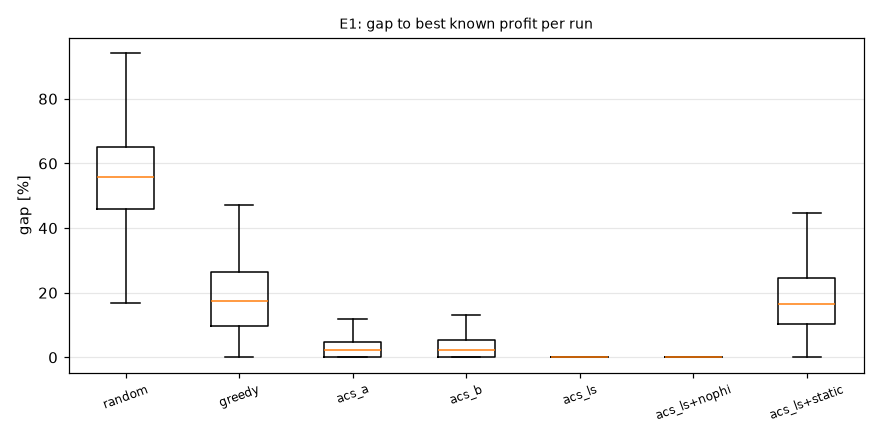
\includegraphics[width=0.85\textwidth]{figures/e1_gap_box.png}
\caption{E1: rozkład luki do najlepszego znanego zysku dla każdej metody.}
\end{figure}

Wnioski:
\begin{itemize}
  \item ACS-LS ma średnią lukę 0,19\%; ACS-A 2,9\%; metoda zachłanna 18,2\%; trasa losowa 54,9\%.
  \item ACS-LS jest lepszy od metody zachłannej na 101 instancjach i nigdy nie jest gorszy, bo zaczyna od trasy zachłannej.
  \item Luka ACS-A rośnie z $N$ i z budżetem. Luka ACS-LS jest prawie stała, bo przeszukiwanie lokalne poprawia kolejność wizyt.
  \item Żadna metoda nie dała trasy niedozwolonej.
\end{itemize}

\textbf{Porównanie z rozwiązaniem dokładnym (K6).} Dla 36 instancji z $N = 25$ CP-SAT (limit 120 s) udowodnił optimum w 24 przypadkach. Średnia luka ACS-LS do najlepszego znanego zysku wynosi 0,09\% (maks. 2,1\%), a na instancjach z dowodem optimum 0,05\%. Najlepsze ziarno ACS-LS osiąga najlepszy znany zysk na 35 z 36 instancji. Dla budżetu 12 h ograniczenie górne CP-SAT jest słabe, więc tam nie ma dowodu optymalności.

\textbf{Mała wyrocznia (K4).} Dla 20 losowych instancji z $N = 7$ program porównał ACS z pełnym przeglądem wszystkich tras. ACS-A z parametrami z dokumentacji ($q_0 = 0{,}9$) znalazł optimum tylko w ok. 63-72\% uruchomień. Przyczyna to krótkowzroczna heurystyka i silna eksploatacja: optymalna trasa często zaczyna się od miejsca o małym zysku, aby inne miejsca odwiedzić w lepszych godzinach. ACS-LS z $q_0 = 0{,}5$ znalazł optimum w 100\% uruchomień. Dlatego ACS-LS jest metodą główną.

\subsection{E2: zbieżność}

\begin{figure}[h]
\centering
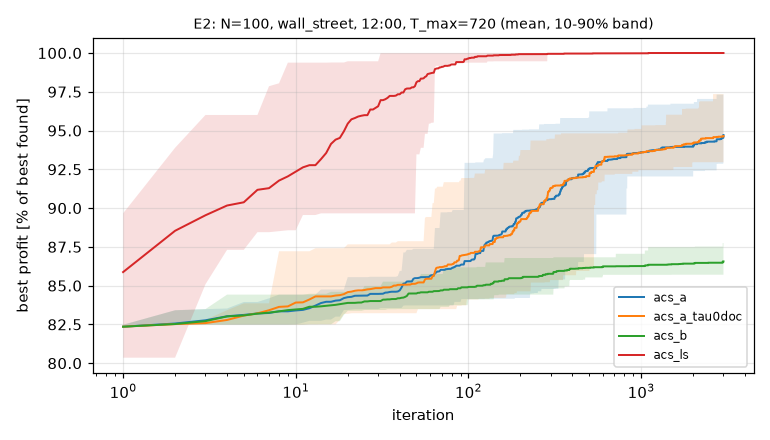
\includegraphics[width=0.8\textwidth]{figures/e2_conv_n100_wall_street_1200.png}
\caption{E2: najlepszy zysk w funkcji iteracji ($N = 100$, Wall Street, 12:00, 12 h; średnia i pasmo 10-90\% z 30 ziaren).}
\end{figure}

\begin{itemize}
  \item ACS-LS osiąga 100\% najlepszego zysku w każdym z 30 uruchomień na dwóch z trzech instancji i 99,7\% średnio na trzeciej. Na instancji z rysunku wystarcza mu ok. 30 iteracji.
  \item ACS-A i ACS-B kończą na ok. 95-98\% po 3000 iteracjach, z dużym rozrzutem między ziarnami.
  \item Wzór $\tau_0$ z pierwszej wersji dokumentacji i wzór $Profit_{greedy}/N$ dają prawie te same krzywe dla ACS-A. Główną przyczyną słabej zbieżności ACS-A jest silna eksploatacja ($q_0 = 0{,}9$) i brak poprawy kolejności wizyt.
  \item ACS-B jest najwolniejszy przy budżecie 12 h (86,6\% najlepszego zysku).
\end{itemize}

\subsection{E3: feromon zależny od pory dnia}

ACS-B ma osobną macierz feromonu dla każdego z 8 przedziałów 3-godzinnych. Na 108 instancjach E1 ACS-B był lepszy 36 razy, równy 29 razy i gorszy 43 razy; różnica nie jest istotna ($p = 0{,}25$). Średnia luka ACS-B jest trochę większa przy każdym budżecie (0,87\% wobec 0,83\% dla 4 h; 5,54\% wobec 5,23\% dla 12 h). Przyczyna: 8 macierzy dzieli te same depozyty na 8 części, więc każda uczy się wolniej, a informację o porze dnia ma już heurystyka $\eta$, która zna godzinę przybycia.

\subsection{E4: wrażliwość parametrów}

\begin{table}[h]
\centering
\caption{E4: efekty główne parametrów ACS-A ($N = 50$, 4 instancje, 30 ziaren; luka do najlepszego zysku dla tej samej instancji i $\lambda$).}
\begin{tabular}{lrrrr}
\toprule
Parametr & Wartość 1 & Wartość 2 & Wartość 3 & Wartość 4 \\
\midrule
$\beta$ & 1: 1,25\% & 2: 1,73\% & 5: 3,39\% & - \\
$q_0$ & 0,5: 1,43\% & 0,7: 1,59\% & 0,9: 2,31\% & 0,98: 3,16\% \\
$m$ & 5: 2,30\% & 10: 2,12\% & 20: 1,95\% & - \\
$\lambda$ & 0,4: 1,39\% & 0,8: 2,53\% & 1,0: 2,45\% & - \\
\bottomrule
\end{tabular}
\end{table}

\begin{table}[h]
\centering
\caption{E4: decyzje projektowe (wzór $\tau_0$, przeszukiwanie lokalne, $q_0$).}
\begin{tabular}{lllrr}
\toprule
$\tau_0$ & Przeszukiwanie lokalne & $q_0$ & Śr. luka [\%] & Maks. luka [\%] \\
\midrule
dokumentacja & nie & 0,5 & 1,18 & 3,85 \\
dokumentacja & nie & 0,9 & 1,85 & 6,53 \\
dokumentacja & tak & 0,5 & 0,46 & 2,76 \\
dokumentacja & tak & 0,9 & 1,38 & 2,76 \\
$Profit_{greedy}/N$ & nie & 0,5 & 0,96 & 2,96 \\
$Profit_{greedy}/N$ & nie & 0,9 & 2,14 & 6,72 \\
$Profit_{greedy}/N$ & tak & 0,5 & \textbf{0,00} & \textbf{0,00} \\
$Profit_{greedy}/N$ & tak & 0,9 & 1,43 & 2,76 \\
\bottomrule
\end{tabular}
\end{table}

\begin{itemize}
  \item Mniejsze $\beta$ i mniejsze $q_0$ dają lepsze trasy. Wartości z literatury dla TSP ($\beta = 2$, $q_0 = 0{,}9$) nie są najlepsze dla tego problemu.
  \item Więcej mrówek daje mały zysk jakości za dłuższy czas obliczeń.
  \item $\lambda$ zmienia funkcję celu: $\lambda = 0{,}4$ daje większy zysk i większy tłok (0,47), $\lambda = 1$ mniejszy tłok (0,35).
  \item Konfiguracja $\tau_0 = Profit_{greedy}/N$ + przeszukiwanie lokalne + $q_0 = 0{,}5$ daje lukę 0\% we wszystkich 120 uruchomieniach. Bez przeszukiwania lokalnego i z $q_0 = 0{,}9$ wzór z dokumentacji jest trochę lepszy, więc wybór $\tau_0$ ma znaczenie tylko w połączeniu z innymi ustawieniami.
\end{itemize}

\subsection{E5: godzina startu}

\begin{figure}[h]
\centering
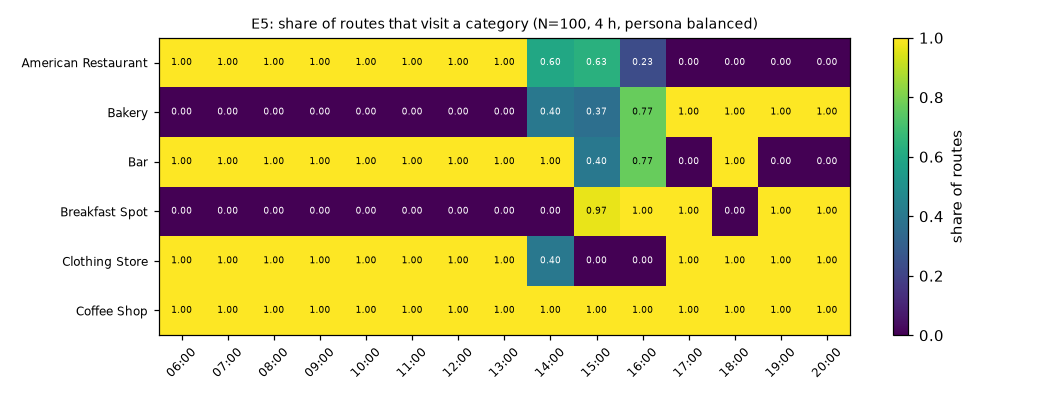
\includegraphics[width=0.95\textwidth]{figures/e5_category_by_start.png}
\caption{E5: udział tras, które odwiedzają kategorię, w zależności od godziny startu ($N = 100$, 4 h, persona ,,Zrównoważony'').}
\end{figure}

Wczesny start (06:00-08:00) i późny start (20:00) dają największy zysk (1,76-1,90) i najmniejszy tłok (0,18-0,28). Start o 17:00-18:00 daje najmniejszy zysk (1,47) i największy tłok (0,48). Trasa dobiera kategorie do pory dnia, ale wykres pokazuje też ważne ograniczenie modelu: persona odwiedza bar przy starcie 06:00-14:00. Bar ma wtedy $P_c = 0{,}06$-$0{,}11$, więc jest ,,otwarty'' według progu 0,05 i prawie pusty. Model nagradza wizytę tuż nad progiem zamknięcia (zob. rozdział o ograniczeniach).

\subsection{E6 i E7: preferencje i punkt startu}

\begin{table}[h]
\centering
\caption{E6: persony ($N = 100$, Times Square, 08:00, 8 h, 30 ziaren).}
\begin{tabular}{lrrrl}
\toprule
Persona & Zysk & Wizyty & Jaccard między ziarnami & Najczęstsze kategorie \\
\midrule
Zrównoważony & 3,28 & 7,0 & 1,00 & American Restaurant, Clothing Store, Bakery \\
Turysta kulturalny & 1,69 & 6,8 & 0,80 & American Restaurant, Park, Coffee Shop \\
Smakosz & 2,91 & 7,0 & 0,85 & American i Mexican Restaurant, Bakery \\
Nocny marek & 2,14 & 7,0 & 1,00 & American i Mexican Restaurant, Bar \\
\bottomrule
\end{tabular}
\end{table}

Kategorie w trasie odpowiadają wagom $u_c$. Trasy są stabilne między ziarnami (Jaccard 0,8-1,0), więc różnice między personami to efekt preferencji. 100 losowych profili $u_c \sim U(0,1)$ daje 67 różnych tras.

W E7 trasy z tego samego punktu startu mają Jaccard 0,78-1,0. Trasy z Times Square, Union Square i Wall Street dzielą część miejsc (Jaccard 0,37-0,65), a trasy z Metropolitan Museum są prawie rozłączne z innymi (0-0,12), bo start jest daleko na północy. Zysk zależy od punktu startu w małym stopniu (1,61-1,76).

\subsection{E8: stabilność danych}

Dla 20 wersji bootstrap i 10 ziaren (200 tras) tylko 2 miejsca (dwie restauracje) są w co najmniej 80\% tras. Trasa zaplanowana na profilu bootstrap i oceniona na profilu z pełnych danych traci średnio 1,2\% zysku (maks. 9,9\%). Model jest dość odporny na szum w danych, ale konkretne miejsca w trasie nie są stabilne.

\subsection{E9: omijanie tłoku}

\begin{figure}[h]
\centering
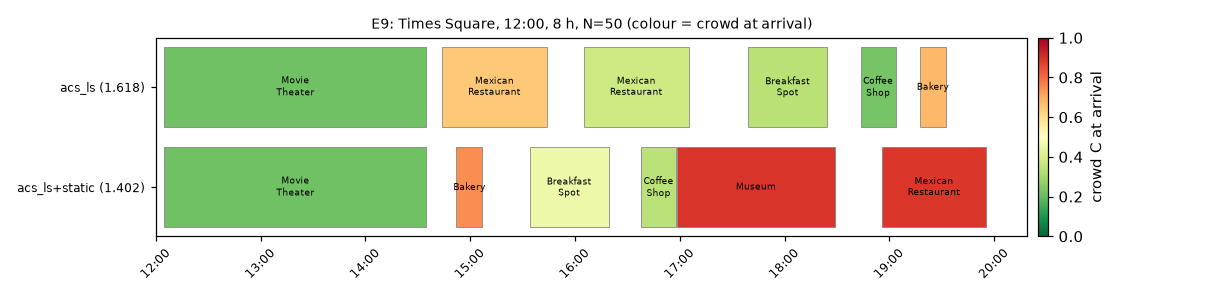
\includegraphics[width=0.95\textwidth]{figures/e9_timeline.png}
\caption{E9: oś czasu trasy z karą za tłok (góra) i bez kary (dół); kolor to tłok w chwili przybycia.}
\end{figure}

Bez kary za tłok średni tłok na trasie rośnie z 0,39 do 0,58, a liczba wizyt w szczycie rośnie z 0,49 do 2,21 na trasę. Tłok jest większy bez kary na 106 ze 108 instancji ($p < 0{,}0001$). Prawdziwy zysk takiej trasy spada do poziomu metody zachłannej (1,27 wobec 1,54). Rysunek pokazuje typowy efekt: trasa bez kary idzie do muzeum o 17:00, w szczycie.

\subsection{E10: zdarzenie znane rano}

Skok tłoku (siła 1, okno 10:00-13:00) trafia w miejsce, które plan bez zdarzeń odwiedza o 10:04: sklep z ubraniami przy starcie 08:00 i meksykańską restaurację przy starcie 10:00.

\begin{table}[h]
\centering
\caption{E10: zysk i koszt zdarzenia ($N = 50$, Times Square, 8 h, 30 ziaren).}
\begin{tabular}{llrrrl}
\toprule
Start & $T_d$ [min] & ACS-LS & Koszt ACS-LS & Koszt \texttt{fixed} & Wizyta ACS-LS w miejscu zdarzenia \\
\midrule
08:00 & 30 & 1,670 & 0,004 & 0,047 & o 14:40 \\
08:00 & 60 & 1,664 & 0,010 & 0,047 & usunięta \\
08:00 & 180 & 1,664 & 0,010 & 0,047 & usunięta \\
10:00 & 30 & 1,656 & 0,101 & 0,187 & o 16:53 \\
10:00 & 60 & 1,652 & 0,105 & 0,188 & o 16:56 \\
10:00 & 180 & 1,648 & 0,109 & 0,189 & usunięta \\
\bottomrule
\end{tabular}
\end{table}

\begin{figure}[h]
\centering
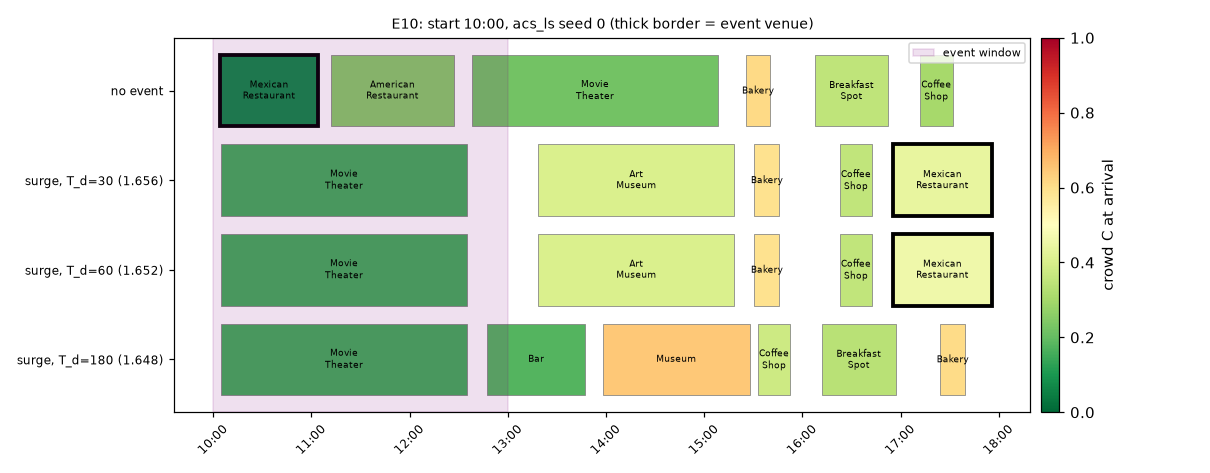
\includegraphics[width=0.95\textwidth]{figures/e10_timeline_1000.png}
\caption{E10: trasa bez zdarzenia i trasy ze skokiem tłoku dla różnych $T_d$ (start 10:00); fioletowe pole to okno zdarzenia.}
\end{figure}

ACS-LS nigdy nie odwiedza miejsca w oknie zdarzenia. Przy krótkim spadku tłoku przesuwa wizytę na popołudnie, przy długim częściej usuwa miejsce z trasy. Plan bez zmian traci ok. 2-12 razy więcej zysku.

\subsection{E11: zdarzenie ogłoszone w trakcie dnia}

Ten sam typ zdarzenia (okno 10:00-13:00, $T_d = 60$ min) trafia w kawiarnię, którą plan poranny odwiedza o 11:56, ale jest ogłoszony dopiero o 11:00. Zysk bez zdarzenia: 1,674. Zysk, gdy zdarzenie jest znane rano: 1,654. Zysk po ponownym planowaniu: 1,647 (ACS-LS) i 1,647-1,648 (ACS-A). Plan bez zmian: 1,517. Ponowne planowanie odzyskuje prawie cały zysk; strata wobec wiedzy od rana to tylko 0,007.

\begin{figure}[h]
\centering
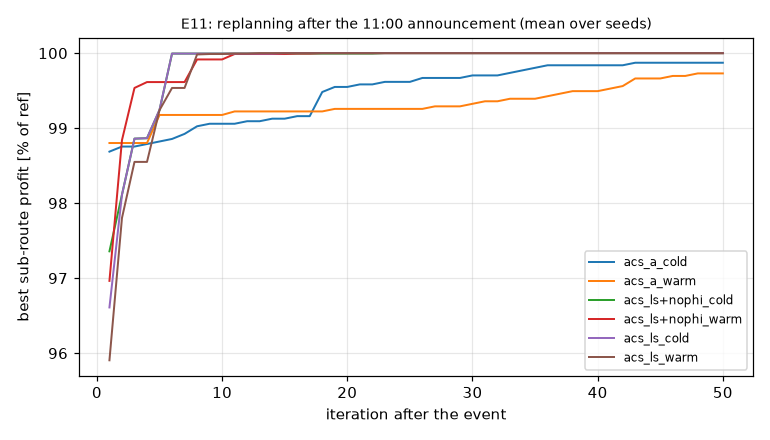
\includegraphics[width=0.75\textwidth]{figures/e11_recovery.png}
\caption{E11: zysk podproblemu po ogłoszeniu zdarzenia w kolejnych iteracjach (zimny i ciepły start).}
\end{figure}

ACS-LS osiąga najlepszy zysk podproblemu w każdym uruchomieniu, średnio w ok. 3 iteracje, z ciepłym i z zimnym startem. Podproblem po 11:00 jest mały (3-4 wizyty), więc ciepły start nie daje tu korzyści. Dla ACS-A ciepły start jest nawet trochę gorszy: stary feromon prowadzi mrówki do starych krawędzi.

\subsection{E12: zamknięcie i parada}

Pierwsze miejsce planu bez zdarzeń (muzeum o 08:24) jest zamknięte 08:00-12:00. Parada przy Times Square (promień 400 m, 12:00-15:00) podwaja czas przejść przez obszar. Zysk bez zdarzeń: 1,674.

\begin{table}[h]
\centering
\caption{E12: zysk i wykonalność tras (30 ziaren).}
\begin{tabular}{lrrrr}
\toprule
Scenariusz & ACS-LS & \texttt{greedy} & \texttt{fixed} & \texttt{fixed} wykonalna \\
\midrule
zamknięcie & 1,643 & 1,460 & 1,674 & 0\% \\
parada & 1,657 & 1,409 & 1,682 & 0\% \\
zamknięcie + parada & 1,616 & 1,460 & 1,682 & 0\% \\
\bottomrule
\end{tabular}
\end{table}

ACS-LS odwiedza zamknięte muzeum po 12:00, gdy jest już otwarte, a koszt zdarzeń jest mały (0,02-0,06). Plan bez zmian jest niewykonalny we wszystkich scenariuszach: wizyta w zamkniętym miejscu albo powrót po czasie przez paradę.

\subsection{E13 i E13b: rola antyferomonu}

W E10-E12 ACS-LS z antyferomonem i bez niego daje prawie zawsze tę samą trasę (176/180, 60/60 i 89/90 remisów). W E1 różnica też nie jest istotna ($p = 0{,}24$).

E13b sprawdza antyferomon w trudniejszych warunkach, w scenariuszu z rozmowy o projekcie: start 09:00 ($N = 100$), zdarzenie ogłoszone o 10:23 i aktywne do 15:00 trafia w przejście, które plan ma zacząć o 11:30. Typy zdarzeń: wypadek (promień 250 m, czas przejścia $\times 50$), zamknięcie miejsca, skok tłoku. Ponowne planowanie ma tylko 10 albo 50 iteracji, z ciepłym albo zimnym startem, dla $\gamma \in \{0, 1, 3\}$. Razem 2160 uruchomień.

\begin{table}[h]
\centering
\caption{E13b: średni zysk całego dnia (30 ziaren).}
\begin{tabular}{llrrrr}
\toprule
Zdarzenie & Metoda & 10 it. zimny & 10 it. ciepły & 50 it. zimny & 50 it. ciepły \\
\midrule
wypadek & ACS-A, $\gamma=0$ & 1,458 & 1,564 & 1,538 & 1,598 \\
wypadek & ACS-A, $\gamma=1$ & 1,445 & 1,548 & 1,563 & 1,596 \\
wypadek & ACS-LS, $\gamma=1$ & 1,582 & 1,619 & 1,605 & 1,622 \\
zamknięcie & ACS-A, $\gamma=0$ & 1,458 & 1,556 & 1,555 & 1,590 \\
zamknięcie & ACS-A, $\gamma=1$ & 1,433 & 1,553 & 1,557 & 1,595 \\
zamknięcie & ACS-LS, $\gamma=1$ & 1,595 & 1,620 & 1,607 & 1,620 \\
skok tłoku & ACS-A, $\gamma=0$ & 1,449 & 1,570 & 1,550 & 1,598 \\
skok tłoku & ACS-A, $\gamma=1$ & 1,447 & 1,564 & 1,551 & 1,602 \\
skok tłoku & ACS-LS, $\gamma=1$ & 1,588 & 1,616 & 1,609 & 1,622 \\
\bottomrule
\end{tabular}
\end{table}

\begin{figure}[h]
\centering
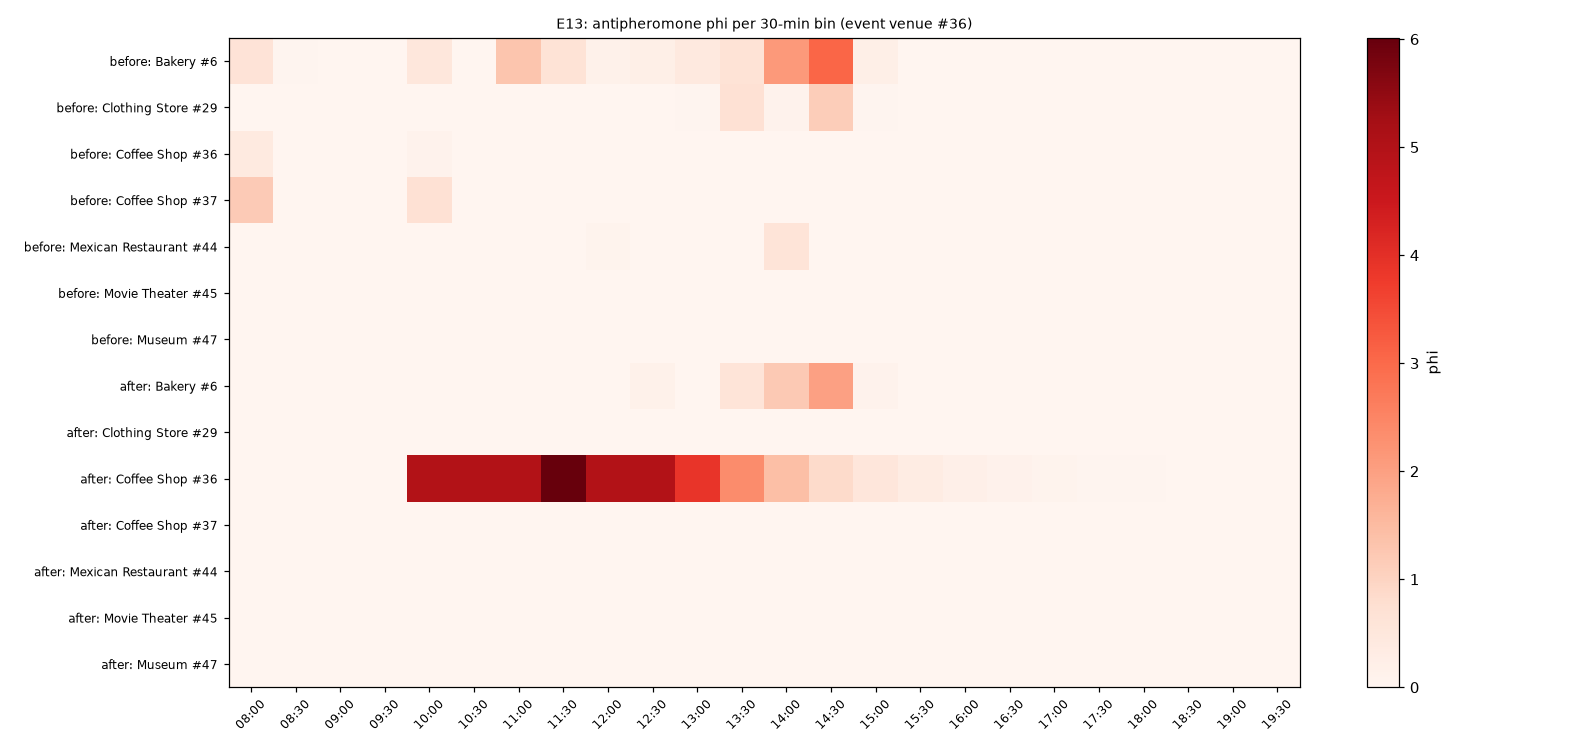
\includegraphics[width=0.95\textwidth]{figures/e13_phi.png}
\caption{Antyferomon przed zdarzeniem i po zdarzeniu (E11): miejsce zdarzenia ma duży $\varphi$ w oknie zdarzenia.}
\end{figure}

Wnioski:
\begin{itemize}
  \item Każdy wariant reaguje poprawnie: 0 tras niewykonalnych w 2160 uruchomieniach, a nowy plan omija zdarzenie.
  \item Antyferomon ze zdarzenia dla wypadku i zamknięcia nie zmienia żadnej trasy (identyczny wynik z wersją bez tych źródeł w 30/30 parach). To wynika z konstrukcji modelu: zamknięte miejsce nie jest kandydatem, a przejście przez obszar wypadku przekracza budżet. Mrówka nigdy nie czyta tego $\varphi$, bo model już zabrania tych wyborów.
  \item $\gamma = 1$ wobec $\gamma = 0$ jest istotnie lepsze tylko w 1 z 12 ustawień; $\gamma = 3$ też nie pomaga.
  \item Ciepły start daje wyraźny efekt przy małej liczbie iteracji: ACS-A po 10 iteracjach ok. 1,55-1,56 wobec 1,43-1,46 przy zimnym starcie. Pamięć kolonii pomaga, ale przez feromon $\tau$, nie przez antyferomon.
  \item Pierwsze uruchomienie E13b ujawniło błąd w ponownym planowaniu: gdy użytkownik szedł do miejsca, które właśnie zamknięto, program zatwierdzał to przejście. Błąd jest poprawiony i ma test regresji.
\end{itemize}

Interpretacja: w obecnym modelu planista zna skutek zdarzenia dokładnie (zakaz, czas przejścia, tłok), więc antyferomon nie dodaje nowej informacji. Antyferomon ma sens, gdy planista zna zdarzenie tylko w przybliżeniu, na przykład ,,wypadek w okolicy, utrudnienia'', bez dokładnego opóźnienia. Wtedy model nie może zakazać wyboru, a antyferomon to jedyny sygnał ,,unikaj tego obszaru''. Ten tryb jest w planie następnej wersji.

% =====================================================================
\section{Ograniczenia i ryzyka}

\begin{table}[h]
\centering
\caption{Ograniczenia wyników.}
\begin{tabular}{p{4.2cm}p{5cm}p{5.2cm}}
\toprule
Ograniczenie & Skutek & Działanie \\
\midrule
Próg zamknięcia $P_c < 0{,}05$ jest za niski & bar rano albo muzeum przed 9:00 są ,,otwarte'' i prawie puste, więc dają prawie pełny zysk; część tras nie jest realistyczna & godziny otwarcia dla kategorii albo z OpenStreetMap (pierwsze zadanie wersji 2) \\
Zdarzenia są symulowane & wyniki E10-E13b nie są pomiarem prawdziwego tłoku & scenariusze ,,co jeśli''; dane opisują tylko zwykły dzień \\
Dane z lat 2012-2013 & profile mogą nie pasować do dzisiejszego miasta & projekt demonstruje metodę, nie jest usługą \\
Check-in to nie liczba gości & profil opisuje aktywność użytkowników Foursquare & $P_c$ to względny wskaźnik tłoku \\
Profil dla kategorii, nie dla miejsca & dwa bary mają ten sam kształt profilu & różnicę daje waga $w_i$ i zdarzenia \\
Brak sieci ulic & przejście to linia prosta $\times 1{,}3$; trasa nie może obejść wypadku inną ulicą do tego samego miejsca & macierz czasów z OSRM (profil pieszy) \\
Wypadek jako mnożnik czasu & zamknięta droga to duży mnożnik, nie pełna blokada & wystarcza dla PoC \\
Przerwane przejście przy zdarzeniu & nowy plan zaczyna się od poprzedniego miejsca, część przejścia jest pomijana & pozycja na odcinku w wersji 2 \\
Brak licencji zbioru & niejasne prawa do publikacji danych & plik źródłowy poza repozytorium, tylko cele akademickie \\
\bottomrule
\end{tabular}
\end{table}

% =====================================================================
\section{Stan prac i plan dalszych prac}

\subsection{Stan obecny}

Pierwsza wersja programu (PoC) jest gotowa: dane, profile, model, ACS ze wszystkimi wariantami, zdarzenia, ponowne planowanie, metody porównawcze, rozwiązanie dokładne, 14 eksperymentów i raport z wynikami. Wszystkie kryteria ukończenia K1-K9 są spełnione. Wizualizacja jest minimalna: wykresy PNG i prosta mapa trasy (folium).

\subsection{Plan wersji 2}

\begin{enumerate}
  \item \textbf{Godziny otwarcia:} tabela godzin dla kategorii albo dane z OpenStreetMap (\texttt{opening\_hours}). To usunie nierealistyczne wizyty tuż nad progiem zamknięcia.
  \item \textbf{Tryb zdarzeń z przybliżoną wiedzą:} planista dostaje tylko antyferomon dla obszaru zdarzenia, a ocena końcowa używa prawdziwego czasu przejścia. Ten tryb pokaże, kiedy antyferomon naprawdę pomaga.
  \item \textbf{Sieć ulic:} macierz czasów przejścia z OSRM, aby trasa mogła obejść wypadek inną ulicą.
  \item \textbf{Wizualizacja:} mapa HTML z suwakiem godziny, animacja feromonu i antyferomonu w kolejnych iteracjach, oś czasu trasy przed zdarzeniem i po nim, opcjonalnie interfejs Streamlit.
  \item \textbf{Symulacja dnia co godzinę:} pętla, która przesuwa użytkownika po planie i planuje ponownie w każdym kroku.
  \item \textbf{Prezentacja wyników} na zajęciach.
\end{enumerate}

% =====================================================================
\section{Podsumowanie}

\begin{itemize}
  \item AntRoute rozwiązuje TDOP z karą za tłok na prawdziwych profilach tłoku z danych Foursquare dla Manhattanu.
  \item Główna metoda (ACS z przeszukiwaniem lokalnym i $q_0 = 0{,}5$) ma średnią lukę 0,19\% do najlepszego znanego rozwiązania i 0,09\% do rozwiązania dokładnego dla 25 miejsc. Metoda zachłanna ma lukę 18\%.
  \item Kara za tłok działa: bez niej średni tłok na trasie rośnie z 0,39 do 0,58.
  \item Ponowne planowanie po zdarzeniu odzyskuje prawie cały zysk, a plan bez zmian często jest niewykonalny.
  \item Ciepły start pomaga przy szybkim ponownym planowaniu. Antyferomon w obecnym modelu nie zmienia wyniku, bo model zna skutek zdarzenia dokładnie; jego rola zostanie sprawdzona w trybie z przybliżoną wiedzą o zdarzeniu.
  \item Najważniejsze ograniczenie to brak godzin otwarcia; to pierwsze zadanie następnej wersji.
\end{itemize}

% =====================================================================
\section*{Bibliografia}
\addcontentsline{toc}{section}{Bibliografia}

\begin{enumerate}
  \item[{[1]}] D. Yang, D. Zhang, V. W. Zheng, Z. Yu, \emph{Modeling User Activity Preference by Leveraging User Spatial Temporal Characteristics in LBSNs}, IEEE Transactions on Systems, Man, and Cybernetics: Systems, 45(1), 129-142, 2015. Zbiór danych: \url{https://sites.google.com/site/yangdingqi/home/foursquare-dataset}.
  \item[{[2]}] M. Dorigo, L. M. Gambardella, \emph{Ant Colony System: A Cooperative Learning Approach to the Traveling Salesman Problem}, IEEE Transactions on Evolutionary Computation, 1(1), 53-66, 1997.
  \item[{[3]}] R. Montemanni, L. M. Gambardella, \emph{An Ant Colony System for Team Orienteering Problems with Time Windows}, Foundations of Computing and Decision Sciences, 34(4), 287-306, 2009.
  \item[{[4]}] J. Montgomery, M. Randall, \emph{Anti-pheromone as a Tool for Better Exploration of Search Space}, ANTS 2002, LNCS 2463, 100-110, 2002.
  \item[{[5]}] M. Guntsch, M. Middendorf, \emph{Pheromone Modification Strategies for Ant Algorithms Applied to Dynamic TSP}, EvoWorkshops 2001, LNCS 2037, 213-222, 2001.
  \item[{[6]}] NYC Open Data, \emph{Borough Boundaries}, \url{https://data.cityofnewyork.us/City-Government/Borough-Boundaries/tqmj-j8zm}.
\end{enumerate}

\end{document}
